\documentclass[a4paper,11pt]{ctexart}

\usepackage{graphicx} 
\usepackage{xcolor}

\usepackage{listings}
\lstdefinestyle{lfonts}{
  basicstyle   = \footnotesize\ttfamily,
  stringstyle  = \color{purple},
  keywordstyle = \color{blue!60!black}\bfseries,
  commentstyle = \color{olive}\scshape,
}
\lstdefinestyle{lnumbers}{
  numbers     = left,
  numberstyle = \tiny,
  numbersep   = 1em,
  firstnumber = 1,
  stepnumber  = 1,
}
\lstdefinestyle{llayout}{
  breaklines       = true,
  tabsize          = 2,
  columns          = flexible,
}
\lstdefinestyle{lgeometry}{
  xleftmargin      = 20pt,
  xrightmargin     = 0pt,
  frame            = tb,
  framesep         = \fboxsep,
  framexleftmargin = 20pt,
}
\lstdefinestyle{lgeneral}{
  style = lfonts,
  style = lnumbers,
  style = llayout,
  style = lgeometry,
}
\lstdefinestyle{python}{
    language = {Python},
    style    = lgeneral,
}

\title{剩余价值率对工人数的两种替代模型——对《资本论》相关替代问题的发掘和发展\newline Two Substitution Models of the Surplus value Rate to the Number of Workers: Exploration and Development of Substitution Issues of Capital}
\author{王苏谈}

\begin{document}

\maketitle
\tableofcontents
\newpage

\begin{abstract}

马克思在考察绝对剩余价值量的剥削问题时,初步研究了剩余价值率对工人数的替代问题,隐约构建了“关于剩余价值总量的剩余价值率对工人数的绝对替代模型”。在这个模型中,所欲维持不变的对象是剩余价值的总量,边界条件是工作日的绝对界限24小时。这个模型对于理解资本家的裁员动机有一定的意义,但存在相当明显的有限性。将模型的维持对象扩大为劳动时间的总量,并通过引入“必要非劳动时间”概念,将其边界缩小为某种相对界限,就形成了“关于劳动时间总量的剩余价值率对工人数的相对替代模型”。后一个模型处于更高环节之上,具有更丰富的规定性。

这二种模型,对于理解资本主义裁减员工、延长工人的劳动时间等经济现象,提供了科学的理论工具,特别是,对于目前常见的一种经验性描述,即减少多少员工并相应地增加单个员工多少工作量等,提供了深刻的理论洞察。相关替代理论具有丰富的理论价值和现实意义,并且为更深入、更全面的研究,诸如相对过剩人口理论,提供了必要的前置环节。

本文深入发掘了马克思《资本论》中有关该替代问题的丰富资源,通过数学的方式准确地描述了二种模型的变动关系,并通过编程的方式形象地表现了相对替代模型的图形。在研究过程中,综合运用了数学和编程的新方法,从而提高了马克思经济学的科学性和说服力。

关键词:剩余价值率;可变资本;工人数;替代模型

When Marx investigates the exploitation of the absolute surplus value quantity, he preliminarily studies the substitution of the surplus value rate for the number of workers, and vaguely constructs "the absolute substitution model of the surplus value rate for the number of workers about the total amount of surplus value". In this model, the object that is desired to remain constant is the total amount of surplus value, and the boundary condition is the absolute limit of working day, 24 hours. This model has some implications for understanding the motivation of capitalists to downsize, but there are rather obvious limitations. By expanding the maintenance object of the model to the total amount of labor time, and by introducing the concept of "necessary non-labor time" and reducing the boundary of the model to a certain relative limit, "the relative substitution model of the surplus value rate for the number of workers about the total amount of labor time" is formed. The latter model is at a higher moment and has richer Bestimmtheit.

These two models provide scientific theoretical tools for understanding the economic phenomena of capitalism, such as reducing employees and prolongating workers' working hours. In particular, they provide profound theoretical insights into a common empirical description, namely, how many employees are reduced and how much work of individual employees is increased accordingly. These substitution theories have rich theoretical value and practical significance, and provide necessary pre-moments for the deeper and more comprehensive studies, such as the theory of relative surplus population.

This paper explores the rich resources of the substitution problem in Marx's Das Kapital, accurately describes the changing relationship of the two models by mathematical methods, and vividly presents the graph of the relative substitution model by programming method. In the process of research, the new methods of mathematics and programming are used comprehensively, thus improving the scientificity and persuasiveness of Marxist economics.

Keywords: rate of surplus value; variable capital; number of workers; substitution models

\end{abstract}

\section{绝对替代模型及其边界条件}

在《资本论》第一卷第九章,马克思在讨论绝对剩余价值的率和量时,论及了剩余价值率对可变资本的一种替代关系:\textit{“因此,在一定量剩余价值的生产上,一种因素的减少可以由另一种因素的增加来补偿。如果可变资本减少,同时剩余价值率却按同一比例提高,那么所生产的剩余价值量仍然不变。”\footnote{卡尔·马克思:《资本论》(第一卷),《马克思恩格斯文集》第5卷,人民出版社2009年版,第352页。下同。}}虽然马克思没有明确将这个问题当作一个模型来讨论,但我们可以将之概括为“关于剩余价值总量的剩余价值率对工人数的替代模型”。

之所以将相关问题归结为替代或替代率问题, 原因之一在于马克思自己在该章所使用的关键的德文词是Ersatz\footnote{MEGA2, Ⅱ/10 (Text), Dietz Verlag, Berlin, 1991, S.274.}(替代),这个词被主流译本翻译成了汉语的“补偿”。这个词在庸俗经济学那里听到的似乎比较多,但从这里应该不难看出,马克思很早就开始分析类似问题了。

为掌握相关模型,应该先了解如下经济关系:

$$\mbox{可变资本的总额} = \mbox{劳动力价值} \times \mbox{工人数}.$$
$$\mbox{剩余价值量} = \mbox{劳动力价值} \times \mbox{剩余价值率}.$$
$$\mbox{剩余价值量的总额} = \mbox{劳动力价值} \times \mbox{剩余价值率} \times \mbox{工人数}.$$

马克思根据上述一些情况,总结出“第一个规律”:\textit{“所生产的剩余价值量,等于预付的可变资本量乘以剩余价值率,或者说,是由同一个资本家同时剥削的劳动力的数目与单个劳动力受剥削的程度之间的复比决定的。”\footnote{《资本论》,第352页。}}

在分析相关问题时,存在如下的一些假设:(一)为购买每个工人所预付的可变资本额$v$在这个模型中保持不变。(二)工人都是抽象同一的工人,他们的劳动力及其价值、劳动强度等皆一致;(三)每个工人的剥削度及其变化方式皆一致。马克思自己亦明确指出了这里所必需的一些条件:\textit{“这里继续假定,不仅一个平均劳动力的价值不变,而且一个资本家所使用的工人已经化为平均的工人。”\footnote{《资本论》,第352页。}}

在这个简单的模型中,工人数是内生变量,它在对单个工人预付的可变资本(=劳动力价值)不变的情况下,并通过这里所说的单个的可变资本,决定了可变资本的总额。剩余价值率是因变量,它之所以发生变动,是为了替代工人数所发生的特定变动。自变量工人数的最典型的变动是减少,相应地,因变量剩余价值率需要提高,以抵消工人数减少后剩余价值量可能的减少。

应该注意到,工人数与可变资本量是二种东西,不能直接等同。但是在这个模型的假设条件之下,工人是均一的,每个工人所得到的工资,即资本家所投入的每一份可变资本,是一样的。因此,在这种条件之下,工人数与工资总额或者说可变资本总额是严格对应的。所以,本文将替代模型中的因变量设定为工人数,是可以接受的。

马克思设计出两个公式,以描述这种替代关系。

$$M = \frac{m}{v} \times V.$$
$$M = k \times \frac{a'}{a} \times n.$$

前一个公式在原理上十分简单,正如马克思所言,个体的剩余价值率即$\frac{m}{v}$乘以总的可变资本量$V$,等于总的剩余价值量$M$。或者亦可以理解为:剩余价值量与可变资本额在总体上与在个体上的两个比值是一致的。与前一个公式相比,后一个公式是从个体的层面加总到整体,即是说,用个体性的诸变量即劳动力价值$k$、剩余价值率$\frac{a'}{a}$、工人总数$n$相乘。

现在已经知道,对于第二个公式而言,在可变资本量(=劳动力价值)不变的情况下,剩余价值总量的影响因素是剩余价值率和工人数,而这二个因素是通过乘积的方式施加影响。以工人数n为自变量,以剩余价值率$\frac{a'}{a}$为因变量,整理上面的这个函数,得剩余价值率对工人数的替代函数如下:$$f(n) = \frac{a'}{a} = \frac{M}{k} \times n^{-1}.$$

然后,上述函数$f(n)$对工人数$n$求导,可得剩余价值率对工人数的替代率函数$$f'(n) = -\frac{M}{k}\times n^{-2}.$$

从上述导函数可知,其值一定是负数,意味着剩余价值率随着工人数的增加而降低,反之,随着工人数的减少而增加;而且,如果深究原函数$f(n)$的二阶导$f''(n) = 2\frac{M}{k}\times n^{-3}$,可知随着减少的工人数越来越多,剩下的工人被剥削的程度越来越高,所需承担的剩余劳动时间也会越来越快地增加。

但无论剩余劳动时间如何增加,它与劳动力价值所代表的必要劳动时间的总和,必定不能超出一个工作日的自然界限,即24小时。因此,上述模型应该从一个工作日的自然界限,设定出来一种绝对的边界条件。只有加上这个边界条件,这个替代模型才成为完整的绝对替代模型。

用方程来描述这个边界条件,得到如下的约束公式:$$\mbox{必要劳动时间} + \mbox{剩余劳动时间} \le \mbox{工作日自然界限}.$$

借助以下公式,剩余劳动时间 = 必要劳动时间 $\times$ 剩余价值率,可得:$$\mbox{必要劳动时间} + \mbox{必要劳动时间} \times \mbox{剩余价值率} \le \mbox{工作日自然界限}.$$

马克思把这个边界条件对这个替代模型所造成的影响,称为“第二个规律”\footnote{《资本论》,第354页。}。工作日的自然界限24小时是绝对不能超出的,否则多出来的劳动时间自然就归为此后的一个或多个工作日。因此,马克思将这类界限称为“绝对的界限”。“平均工作日天然地总是少于24小时,它的[这个]绝对的界限,对于替代减低的可变资本以提高的剩余价值率,或者[替代]减少的受剥削的工人数以增加的剥削度,构成一种绝对的界限。”\footnote{参阅MEGAII/10. S. 275. 参阅《资本论》,第354页。这里的引文是根据德文版重译的。}。实际上,只有加上这个边界条件,这个模型在相应的叙述环节上才是完整的。

将前面的一些参数代入这个公式,可得如下方程:$$v + v \times \frac{a'}{a} \le 24.$$解得:$$\frac{a'}{a} \le \frac{24}{v} - 1.$$再代入劳动力价值$v = 6$,得$\frac{a'}{a} \le 3$。所以,在马克思所设计的绝对替代模型中,代入给定的诸参数,并受到边界条件的约束后,可知,作为替代因素的剩余价值率的边界是3。

\section{绝对替代模型的意义和有限性}

为理解这个绝对替代模型的特定意义,我们可以讨论马克思所说的一种趋势,即\textit{“资本要尽量减少自己所雇用的工人人数即减少转化为劳动力的可变资本部分的趋势”\footnote{《资本论》,第354页。}}。绝对替代模型所着重强调的内容,就是资本家可从这种可变资本的减少中获益。

在该模型中,剩余价值的总量是不变的,在这个方面资本家没有得到什么更多的东西,然而由于剩余价值率的提高可以替代工人数的减少,资本家会从这两个变动中的后一个上面,得到一个明显的好处,即减少预付给工人的可变资本部分,节省下来的这部分资本可以通过不同的方式来更大地增殖资本。可以可变资本节省公式来理解这个经济过程如下:$$\mbox{节省的可变资本} = \mbox{可变资本} \times \mbox{裁员数}.$$

绝对替代模型有其特定的理论意义,但它同样有着很大的局限性。

马克思的绝对替代模型,只借用了比较简单的概念,试图反映一些极抽象环节上的关系。但是,这些关系在现实中能否按其本身的抽象方式得以实现,甚至都是有严重的疑问的。比如,资本家在实际地调整工人数的时候,不是以剩余价值量为依据,而是直接以劳动时间总量为依据等等。在这样的情况下,较抽象环节上的规律就更难直接地肯定。它们要在现实中发挥具体作用, 就需要经过更多的、更曲折的中介,甚至,就这个特定的替代问题而言,或许不能保有其任何意义上的实存。因此,该模型或许更多地是具有科学体系里特定环节上的真理之意义。

另外,由于缺乏相应的数学工具,《资本论》相关章虽然能指出绝对替代模型中剩余价值率与工人数之间存在某种替代关系,但无法指认出二者之间的精确的替代率函数,即对相应的替代函数求导得出的导函数。

而且由于所涉的参数比较稀薄、单调,这个模型的理论意义同样比较有限。主要应该考察该模型的维持不变的对象和边界条件这二个方面。

首先,在马克思的这个绝对替代模型中,剩余价值率与工人数互相替代时应该维持的对象,是那个原有的剩余价值总量$M$。然而在更具体、更真实的经济关系中,资本家考虑的类似问题却是:在劳动时间总量保持不变的情况下,如何通过剩余价值率的提高来替代工人数的减少。因此,在更具体的模型中,或者说在更高的环节上,应该考虑的问题是:在维持劳动时间总量不变的情况下,剩余价值率与工人数的替代关系。

其次,从工作日的界限的角度来看,24小时确实是工作日的绝对界限。但是无论如何,一般地,劳动者都必须保持一个必要的睡眠时间,以再生产自身的劳动能力,此外劳动者还需要休闲、娱乐、学习、养育后代等的时间。因而总的看来,工人还需要一个必要的不进行劳动的时间,处于无论是必要劳动时间还是剩余劳动时间之外。于是,可以设想在工作日的绝对界限之内,还有一个因素即\textit{必要非劳动时间},导致了更严的界限。这个界限受到社会阶段、风俗习惯、阶级斗争、劳动法律法规等方面的多重影响,因此它是一个相对的界限。不过我们在考察它的时候,可以假定它在短期甚至中期内是可以保持不变的。

将模型所欲维持不变的对象,从剩余价值总量替换为更大的劳动时间总量,将模型中的界限,从工作日的绝对界限替换为更窄的工作日的相对界限,就可以形成一个更具体的、更贴近现实的替代模型——“关于劳动时间总量的剩余价值率对工人数的相对替代模型”(以下简称“相对替代模型”)。

\section{相对替代模型及其边界条件}

为了构建相对替代模型,需要先了解一些基本的数学关系。
$$\mbox{劳动时间总量} = \mbox{工人数} \times\mbox{(必要劳动时间 + 剩余劳动时间).}$$
$$\mbox{剩余劳动时间} = \mbox{必要劳动时间} \times \mbox{剩余价值率}.$$

联立上述二个方程,消去剩余劳动时间这个参数,并以工人数为自变量、以剩余价值率为因变量加以整理,可得剩余价值率对工人数的相对替代函数如下:

$$\mbox{剩余价值率} = \frac{\mbox{劳动时间总量}}{\mbox{必要劳动时间}} \times \mbox{工人数}^{-1} - 1.$$

在上面的相对替代函数中,主要是从劳动的层面设定相关参数,而这里的必要劳动时间在价值上就代表着可变资本,这里的剩余劳动时间就代表着剩余价值,如此等等。劳动时间总量、必要劳动时间是外生变量,工人数是自变量,剩余价值率是因变量。在相对替代模型的限度内,由该公式可以得知剩余价值率对工人数在数学上的精确的替代关系。对比此前的绝对替代模型中的相应替代关系,可见原来的剩余价值总量被替换成了劳动时间总量,并且新的公式中有一个$-1$,这是由于必要劳动时间也被纳入模型的考察范围。

设剩余价值率 = 1/2,工人数 = 100人,必要劳动时间 = 6小时。可得剩余劳动时间 = 3小时,劳动时间总量 = 900小时。现在,比如说裁员20人,剩下100 - 20 = 80人,由上述相对替代函数可得剩余价值率 = 0.875。则对于单个劳动者而言,剩余劳动时间 = 必要劳动时间 $\times$ 剩余价值率 = 5.25小时,每工作日的工作时长 = 必要劳动时间 + 剩余劳动时间 = 11.25小时。相比此前的工人数下的情况,现在每个工人需要多劳动的时间 = 5.025 - 3 = 2.25小时;相反,资本家节省下来的可变资本换算成的劳动时间 = 必要劳动时间 $\times$ 裁员数 = $6 \times 20$ = 120小时。

这里实际上假设了资本家不会为工人的延长劳动时间而额外支付报酬。所以,在节省可变资本的这个经济规律的影响下,资本家会拼命地“减员增效”,降低用工成本。相应地,如果存在加班工资等因素的影响,这个规律就会在一定程度上变形。

更进一步,相对替代函数对工人数求导,可得剩余价值率对工人数的相对替代率如下:$$\frac{d\mbox{剩余价值率}}{d\mbox{工人数}} = -\frac{\mbox{劳动时间总量}}{\mbox{必要劳动时间}} \times \mbox{工人数}^{-2}.$$

该相对替代函数的导函数表示,在给定的劳动时间总量和必要劳动时间下,工人数的变动会如何影响剩余价值率的变动。这个公式的值为负,意思是:在相应条件下,当工人数增加时,剩余价值率就会减少;反过来理解,当工人数减少时,剩余价值率就会增加。后者才是绝对替代模型和这里的相对替代模型所关注的典型情况。并且,工人的人数减得越少,剩余价值率就越需要提高。延续并代入此前的一些参数,可得:$$\frac{d\mbox{剩余价值率}}{d\mbox{工人数}} = -150 \times \mbox{工人数}^{-2}.$$

在相对替代模型中,也存在一个相对的边界条件或者说约束条件。我们此前已经设定工人必须有一个“必要非劳动时间”。那么可知一个如下的相对约束公式:$$\mbox{必要劳动时间} + \mbox{剩余劳动时间} \le 24 - \mbox{必要非劳动时间}.$$

借助下面的这个常用的公式,剩余劳动时间 = 必要劳动时间 $\times$ 剩余价值率,并设定必要非劳动时间为9小时,则从该相对约束公式可得:$$6 \times (1 + \mbox{剩余价值率}) \le 24 - 9.$$解得剩余价值率 $\le$ 1.5。再将这个解及其他相关参数代入剩余价值率对工人数的相对替代函数,求得边界上的工人数为60人。这意味着:在原工人数100人、必要劳动时间6小时、必要非劳动时间9小时、劳动时间总量900维持不变的情况下,最大的剩余价值率是1.5,最多能裁员到60人。

在相对替代模型中,还存在一个十分隐蔽却又十分重要的副作用。在初始状态下,劳动时间总量的900中有比如600的必要劳动时间的总量和300的剩余劳动时间的总量,然而比如在以上所得的边界上,必要劳动时间的总量 = 必要劳动时间 $\times$ 工人数 = 6 $\times$ 60 = 360,此时为了达成该模型所欲维持的劳动时间总量900,则剩余劳动时间 = 劳动时间总量 - 必要劳动时间的总量 = 900 - 360 = 540。就是说,在维持劳动时间总量不变的情况下,不仅剩余价值率,而且剩余劳动时间的总量即剩余价值的总量,都不得不随着工人数的减少而增加。从替代率函数上看,在经济环境相同的情况下,相对替代模型所欲维持的劳动时间总量大于绝对替代模型所欲维持的剩余价值总量,则相对替代模型的替代率函数的系数的绝对值更大,剩余价值率的变动更大。从实际层面来看,增加的这部分剩余劳动时间,是用于替代裁掉的工人所对应的那部分必要劳动时间。

总的来看,相对替代模型在保证了原有的劳动时间总量的前提下,既可以减少可变资本的预付,还可以同时提高剩余价值的率和量。\iffalse 再苦一苦工人阶级吧……\fi

\section{相对替代模型的程序化和可视化}

为了直观地了解该替代模型中作为替代因素的剩余价值率和作为被替代因素的工人数之间的相互关系,可设计一份相关的Python程序如下:

\begin{lstlisting}[style = python]
import matplotlib.pyplot as plt\textsc{}
import matplotlib as mpl


def getSurplusLabourRate(work_time_sum, worker_num, necessary_labour_time):
return (work_time_sum / (worker_num * necessary_labour_time)) - 1


work_time_sum = 900
necessary_labour_time = 6
worker_num_orig = 100

worker_num_list = list(range(worker_num_orig, int(worker_num_orig / 2), -1))
surplus_labour_rate_list = [
getSurplusLabourRate(work_time_sum, worker_num, necessary_labour_time)
for worker_num in worker_num_list
]

cmap = mpl.colors.ListedColormap(["DeepSkyBlue", "Coral", "Crimson", "#DCDCDC"])
norm = mpl.colors.BoundaryNorm([0.5, 0.8, 1.20, 1.5, 2.0], cmap.N)
colors = cmap(norm(surplus_labour_rate_list))

cmap.set_under("black")
cmap.set_over("grey")

plt.scatter(
worker_num_list,
surplus_labour_rate_list,
c=colors,
cmap=cmap,
norm=norm,
)
plt.colorbar(mpl.cm.ScalarMappable(norm, cmap), extend="both")

plt.show()


\end{lstlisting}

这份代码设定的劳动时间总量work\_time\_sum为900,必要劳动时间为6,原本的工人数为100。现在我们假定工人数每次减少1名,直至减少到51名。工人数的数据保存在列表worker\_num\_list。从这些数据可以依次计算出相应的剩余价值率\footnote{代码中是规定为“剩余劳动率”,因为这是从劳动的层面来看剥削度,其实它等于剩余价值率。},保存到列表surplus\_labour\_rate\_list。将这两个列表分别当作横纵坐标上的值并对应起来形成若干点的坐标,由此做散点图。该图中的点的颜色,经过特殊的处理,以表明它们处于特定的数值区间。所得到的散点图如图1所示。

\begin{figure}[htb]
    \centering
    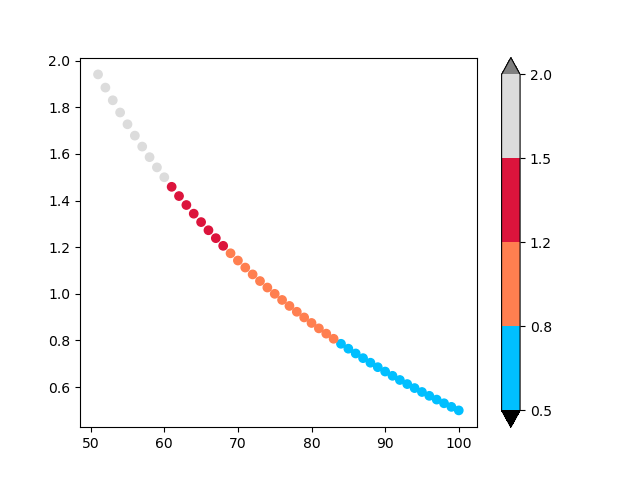
\includegraphics[width=\textwidth]{Figure_1.png}
    \caption{\label{1} 关于劳动时间总量的剩余价值率对工人数的相对替代模型散点图}
\end{figure}

图形表现为散点图,因为工人的数量是自然数,但是这些点确实都位于相对替代函数上,并且从极限的角度来理解,无数的数据点可以形成一条极为光滑的曲线。

从这个散点图可知,在控制其他变量的情况下,为了维持原有的工作量,若工人数减少,则剥削度要加强,若工人数增加,则剥削度会减轻。被裁的工人越来越多(横坐标从右往左看),则剩余价值率就要上升,意味着剩下的工人之工作时间被逐步增加,他们越来越辛苦,点的颜色相应地变得更有刺激性。但是,剩余价值率若上升到超出1.5,即我们此前计算所得的剩余价值率之边界,则点的颜色就变成淡的了,意思是:在既定的必要非工作时间的约束下,工作时长已经超出了工人的忍耐极限,因而不能实行。在边界上能实现的最少工人数是60名,就是说,裁掉了40名工人。

对资本家来说,在维持完成原有工作量的基础上,只要能减少工人数,就能节省可变资本上的支出。因此,在该模型中,工人数会不断减少,尽可能接近其所能达到的极限。即是说,尽可能裁掉一部分工人,在剩下的工人还能忍受的情况下,相应地延长其工作时间。

从函数图像不难得出一些次要的或派生的结论。诸如,在相对界限之内,如果有一个点位于相对替代函数所形成的曲线之上,就意味着在这个点所对应的工人数的情况下,剥削程度相对地更大了,所获的剩余价值相对地会更多;反之,如果在该曲线之下,就意味着在相应的工人数的情况下,剥削度更少地提高,从而所获的剩余价值相对地会更少。由于资本家更多地榨取剩余价值的动机,曲线之下的点存在希望上升的动机,曲线之上的点存在抗拒下降的动机。

\section{结论}

马克思的、并由本文加以规范化的关于剩余价值总量的剩余价值率对工人数的绝对替代模型,讨论的是:以剩余价值总量为维持对象,以工作日的绝对界限为边界时,剩余价值率的提高如何替代工人数的减少。本文所设计的关于劳动时间总量的剩余价值率对工人数的相对替代模型,讨论的是:以劳动时间总量为维持对象,以工作日的某种相对界限为边界时,剩余价值率的提高如何替代工人数的减少。

这些模型都把节省可变资本投资作为自己内在的动机,把裁员和延长工作时间作为实现这一动机的手段。因此,这些模型都侧重于观察工人数减少而不是增加的情况下剩余价值率的替代情况,目的在于展现资本家减少可变资本投资的经济动机,然而都能覆盖这二种情况。

这两个模型都排除了其他的一些复杂因素的影响,比如它们都排除了劳动强度的差别,将这些时间里的劳动强度视为均一的。

然而与绝对替代模型相比,相对替代模型扩大了所欲保持的劳动量之范围,缩小了替代效应起作用的边界,在这两个方面都有所发展。相对替代模型因为更加接近具体的总体,所以应该属于理论上的更高环节。它对此前的极抽象环节上那些看似固定的、无暇的东西,是进行了否定,但同时也是肯定了其中的有现实性的内容。

通过这二个模型,可以在特定方面上更深刻地理解资本主义减少工人数、延长工人的劳动时间等的内在经济动机,并为理解更高环节上的其他相关经济规律,打下坚实的理论基础。

比如,传统的相对过剩人口理论的核心依据,是资本有机构成之提高。并且,资本对劳动力的需求存在边际递减。然而,考虑到这里所阐发的剩余价值率对工人数(可变资本)的替代模型,相对过剩人口的传统解释就显得特别片面。因为,不仅资本有机构成之提高,而且剩余价值率对工人数(可变资本)的替代,也会导致相当多的工人从生产过程中游离出来。相比而言,前者更具有固定性,后者更具有灵活性。因为,比如就相对替代模型而言,首先,资本家所能达到的替代程度是比较灵活的,存在一个活动的区间,其次,工作日的相对界限是相对的、容易变动的。在考虑有关替代模型在相对过剩人口理论中的作用时,应该注意:在实际的经济观察中,替代模型已经发挥作用,就是说,直接观察到的工人数,或者说固定资本与可变资本的若干比例云云,已受到替代模型的动态影响。

然而即便是第二个更具体的模型,也可通过放宽或引入特定的诸参数而更加具体化。不同的模型之间还有复杂的相互作用,诸如此类。不是把这些模型当成固定的、死板的东西,而是看作不同环节上的有限而又有合理性的东西,才能准确地把握它们的规定性。

\end{document}
